
\documentclass{article}
\usepackage{pgfplots}
\pgfplotsset{compat=1.18}
\usepackage{amsmath}

\begin{document}

\begin{center}
% First Normal Distribution (centered at 0)
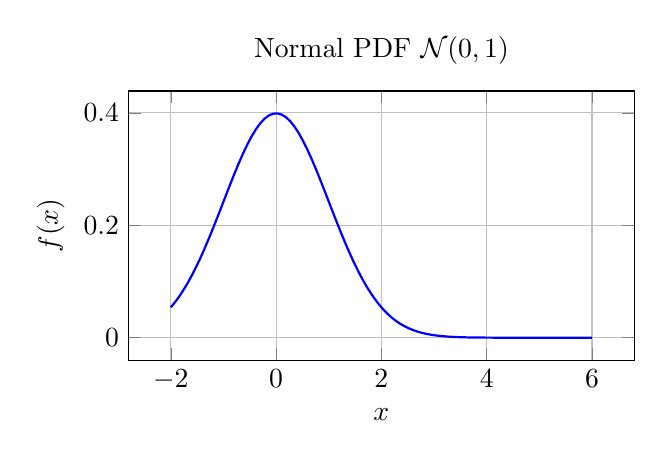
\begin{tikzpicture}
\begin{axis}[
    title={Normal PDF $\mathcal{N}(0,1)$},
    xlabel=$x$, ylabel=$f(x)$,
    domain=-2:6, samples=100,
    width=8cm, height=5cm,
    grid=both,
]
\addplot[
    thick,
    blue,
]
{1/sqrt(2*pi) * exp(-x^2/2)};
\end{axis}
\end{tikzpicture}

\vspace{1cm}

% Second Normal Distribution (centered at 3)
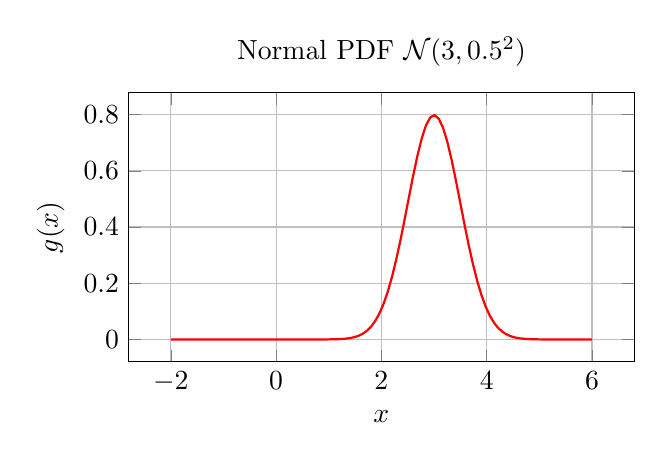
\begin{tikzpicture}
\begin{axis}[
    title={Normal PDF $\mathcal{N}(3,0.5^2)$},
    xlabel=$x$, ylabel=$g(x)$,
    domain=-2:6, samples=100,
    width=8cm, height=5cm,
    grid=both,
]
\addplot[
    thick,
    red,
]
{1/(0.5*sqrt(2*pi)) * exp(-(x-3)^2/(2*0.5^2))};
\end{axis}
\end{tikzpicture}

\vspace{1cm}

% Convolution (N(0,1) * N(3,0.5^2) = N(3, 1.25))
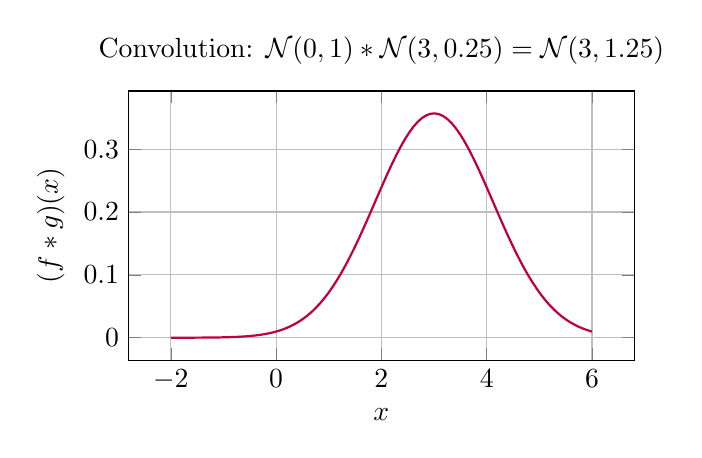
\begin{tikzpicture}
\begin{axis}[
    title={Convolution: $\mathcal{N}(0,1) * \mathcal{N}(3,0.25) = \mathcal{N}(3,1.25)$},
    xlabel=$x$, ylabel=$(f*g)(x)$,
    domain=-2:6, samples=100,
    width=8cm, height=5cm,
    grid=both,
]
\addplot[
    thick,
    purple,
]
{1/sqrt(2*pi*1.25) * exp(-(x-3)^2/(2*1.25))};
\end{axis}
\end{tikzpicture}

\end{center}

\end{document}

